\documentclass[pageheader,chapter,shorttitle,mathtxf]{njubachelor}

\sid{091120000}
\grade{09}
\cauthor{曹增乐}
\ctitle{南京大学本科毕业设计 \LaTeX{} 模板}
\cdepartment{物理学院}
\cspecialization{物理基地}
\cmentor{老板}{教授}
\ckeywords{南京大学; 本科毕设; \LaTeX{} 模板}
\cdate{2013年2月24日}

\eauthor{Zengle Cao}
\etitle{\LaTeX{} Template for Bachelor's Thesis of Nanjing University}
\edepartment{School of Physics}
\especialization{Physics}
\ementor{Boss}{Prof.}
\ekeywords{Nanjing University (NJU); Bachelor's Thesis; \LaTeX{} Template}

%\includeonly{chapters/chapter3}

\begin{document}

\makectitlepage

\begin{cabstract}
这是中文摘要。
\end{cabstract}

\begin{eabstract}
This is English abstract.
\end{eabstract}

\frontmatter
\pagenumbering{Roman}

\maketoc

\mainmatter


\makectitle

\chapter{\LaTeX{} 之我见}

\section{工具与艺术}

之前在人人上看到一篇介绍 \LaTeX{} 的文章,
第一句话说的便是
\begin{quotation}
  \it \LaTeX{} 并不难, \LaTeX{} 也不是艺术。
\end{quotation}
对此,我并不完全赞同。
诚然,对于一部分,甚至是很大一部分人来说
\LaTeX{} 的确只是一个写文章的工具,
但其底层 \TeX{} 设计的初衷绝非仅限于此。

\TeX{} 之父,正是有编程圣经之称的 {\it The Art of Computer Programming\/} 的作者,
大名鼎鼎的 \textit{Donald E. Knuth\/} 教授。
他在为 \TeX{} 系统撰写的手册 \textit{The TeXBook\/} 第一章便写道

\begin{quotation}
  \small
  English words like `technology' stem from a Greek root beginning with
  the letters $\tau\epsilon\chi\ldots\,$; and this same Greek word means {\sl
  art\/} as well as technology. Hence the name \TeX, which is an
  uppercase form of $\tau\epsilon\chi$.
  
  \begin{center}
      \ldots\ldots\ldots\ldots\qquad
      \ldots\ldots\ldots\ldots\qquad
      \ldots\ldots\ldots\ldots\qquad
      \ldots\ldots\ldots\ldots\qquad
      \ldots\ldots\ldots\ldots
  \end{center}
  
  The purpose of this pronunciation exercise is to remind you that \TeX\ is
  primarily concerned with high-quality technical manuscripts: Its emphasis is
  on art and technology, as in the underlying Greek word. If you merely want
  to produce a passably good document---something acceptable and basically
  readable but not really beautiful---a simpler system will usually suffice.
  With \TeX\ the goal is to produce the {\sl finest\/} quality; this requires
  more attention to detail, but you will not find it much harder to go the
  extra distance, and you'll be able to take special pride in the finished
  product.
\end{quotation}
足见 \TeX{}/\LaTeX{} 并不仅仅是工具而已,它的诞生就是为了满足高质量排版的各种苛刻要求。

又或者说,\LaTeX{} 本身是一种工具,而排版是艺术。
就好比一支笔。很多人用笔写字,只是为了记录和表达,于他们而言,笔仅仅是工具。
但也有人,成了书法家,书法是一种艺术。
要写得好字,功夫自是必不可少的,一支好笔也同样很重要。
\LaTeX{} 对于排版艺术,就是一支好笔。


\section{软件与语言}

就好比 C++ 是一种编程语言,而微软的 VC++ 是开发环境,它只是为了提高效率而已。
没有 VC++,还可以选择 devC++,或者使用任何文本编辑器配合编译器。
语言的核心,只是代码和编译器而已。

同样的,虽然很多人把 \LaTeX{} 视为软件,私以为以排版语言理解之更为合适。
其实只需一个编辑器编辑源文件,在命令行里编译,就可以得到高质量的排版结果。
而所说的软件,如 \CTeX 套装里自带的 WinEdt,以及开源的 TeXworks,TeXstudio 等,
就好比 VC++ 或者 devC++。
所以说,\LaTeX{} 其实是一种编译器,或者语言。
正如 C++ 编译器用来编译 C++ 语言,当谈论 \LaTeX{},我们既指编译器,也指语言。

当然,令人惊奇的是,当我们谈论 \LaTeX{},很多时候我们用的却并非在用 \LaTeX{} 进行编译。
首先,我们应该先搞清楚 TeX,pdfTeX,XeTeX 以及 LaTeX,pdfLaTeX,XeLaTeX。
当然,继续了解,还有 ConTeXt,LuaTeX 等。
比如 TeX,pdfTeX,XeTeX,是 TeX 的三种编译器,它们共同编译满足 TeX 语法的源文件。
不同的是 TeX 输出的是~.dvi 格式的文件,需要经过额外的转换才能得到 pdf 文件。
要知道,TeX 的诞生可比 pdf 的流行要早得多。
而 pdfTeX,顾名思义,可以直接输出 pdf 文件。
TeX 系统原本并不支持调用操作系统字体,它调用的字体都是 TeX 系统自带的文件定义的,
而标准的 LaTeX 发行版,因为版权原因并没有包含 windows 上常用中易字体的定义文件。
另一方面,原先的 TeX 系统只具备处理标准 ASCII 码的能力,
对于中文这样字符数量庞大的语言,就更加无法提供支持了。
虽然 TeX 系统诞生之出并不支持非英文语言,
但在世界各地用户的努力下,TeX 系统也开始支持越来越多的语言。
至于 XeTeX,则可以调用系统字体,并且使用通用性更好的 UTF-8 编码,让非英文排版变得简单。
再说说我们的主角 LaTeX,原本只是基于 TeX 的一个拓展。
它的语法与 TeX 并不兼容。虽然 TeX 文档和 LaTeX 文档的后缀都是~.tex,
但既不能用 TeX 编译器编译 LaTeX 源文件,也不能用 LaTeX 编译器编译 TeX 源文件。
LaTeX 和 ConTeXt,LuaTeX,都是 TeX 的拓展。
LaTeX 是其中最流行的拓展,另外两个不甚了解,就不作介绍了。
这里已经不难理解 pdfLaTeX 和 XeLaTeX,分别是 pdfTeX 和 XeTeX 向上兼容 LaTeX 拓展的产物了。

当然 \LaTeX{} 现在已经是一个很笼统的称呼了。
一个完整的 \LaTeX{} 发行套装,包含上述提到的全部编译器,
甚至还提供了 \texttt{metapost} 和 Asymptote 这样强大的绘图语言。
另外 windows 版本还会自带编辑器。
而我们最常用的还是 \LaTeX{} 语言和它相应编译器。
由于以前用 Linux 时 LaTeX 和 pdfLaTeX 还不能处理中文,
我自己对 XeLaTeX 情有独钟,
以至于这份模板仅支持 XeLaTeX 一种编译途径。


\section{\LaTeX{} 与 Word}

\LaTeX{} 与 Word 的差别,
其实就是一个开源的可扩展的排版语言,
和一个封闭的商业软件的差别。

首先,作为一种排版语言,\LaTeX{} 体现出了惊人的可扩展性。
只要有人为它开发宏包,它就能拥有很多令人吃惊的功能。
除了自带的优秀的公式排版,它还可以借助相应的宏包排版
化学结构式、流程图、交换图,甚至各种棋谱和乐谱。
使用 Word,你需要另外购买的功能,\LaTeX{} 很多都可以通过宏包实现拓展。

同时,作为排版语言,\LaTeX{} 让你可以通过命令对排版效果进行细致的控制。
就比如上边这段话,我们可以试着在“甚至各种棋谱和乐谱。”
后加上 \verb|\linebreak| 命令来建议 \LaTeX{} 断行。
得到的效果如下边这段话:

首先,作为一种排版语言,\LaTeX{} 体现出了惊人的可扩展性。
只要有人为它开发宏包,它就能拥有很多令人吃惊的功能。
除了自带的优秀的公式排版,它还可以借助相应的宏包排版
化学结构式、流程图、交换图,甚至各种棋谱和乐谱。\linebreak
使用 Word,你需要另外购买的功能,\LaTeX{} 很多都可以通过宏包实现拓展。

在 Word 里没有这样的自由吧,是不是很赞!再看看这个,如果我要输入公式
\begin{gather*}
  -x<y<z \\ p<y<z
\end{gather*}
这样的效果似乎还不够,在 $p$ 前加入 \verb|\phantom{-}| 占据一个负号的位置呢?
\begin{gather*}
  -x<y<z \\ \phantom{-}p<y<z
\end{gather*}
我想这就是工具与艺术的区别!

\LaTeX{} 另外个巨大的巨大的优势就在于用
\verb|\chapter{}|,\verb|\section{}| 这样的命令来整理文章的逻辑结构,
通过预先定义章节标题的样式来实现各种效果。
试想一下 Word 里,你打了“1. 标题”,然后回车准备输入正文,这时候出现了自动编号。
可是下一节写什么你还没有想好啊,于是退格删除,把格式改回正文的格式。
打到下一节,输入“2. 标题”,再用格式刷把第一节的标题刷到第二节。
为了让标题与上一段分开一点,你在上一段末尾多敲了一个回车。
有时候还会遇到更尴尬的情况,这个标题正好在一页的末尾,这一节就这样被“斩首”了,
不太好看,于是你回到上一节,啪啪啪一路回车愣是把这一节的标题换到下一页。
接着写,你突然想起来前面要再插入一节。
如果你不太清楚大纲视图和自动编号,那惨了,你得把后面的节前面的数字全部改了。
别忘了还有你之前换页敲的一溜回车,重新删了吧……

好吧,我又在意淫 Word 用户的困扰了。
其实我并不是要黑 Word,只是拿全靠回车、空格和格式刷排版的 Word 用户举个例子。
习惯了 \LaTeX{} 的 \verb|\chapter{}|,\verb|\section{}|这一套,
回到 Word,便会自觉地开始学习用样式来规定标题的格式和编号,
标题设置成与下段同页就避免了上述的尴尬,
孤行控制还可以防止某段的最后一行落到下一页,诸如此类。
当习惯了 \LaTeX{} 通过 \verb|\label{}| 和 \verb|\ref{}| 统一地实现交叉引用,
回到 Word,就会学习使用题注来添加图表标题。
当然,你最终会发现,这些没有 \LaTeX{} 里的命令来得好用。

这便是 \LaTeX{} 所谓“所想既所得”与 Word 之“所见即所得”的差别。
\LaTeX{} 让你专注于写文章,而非文章的排版。
我想很多人之所以把 \LaTeX{} 视为工具,原因就在于此。
既然不需要写文章的人关注排版,那么事先定义好详细的排版规则,
让排版出来的文章美观、高质量,这就是 \LaTeX{} 和其它宏包设计者该做的事了。
对于这些人,\LaTeX{} 必须是艺术。
当然,前面给出的两个关于细节控制的例子,
对于将 \LaTeX{} 完全视为工具的使用者而言,是不必要了解的,
对于重视排版效果的人,则会为这个系统贴心的设计感到欣喜。

写了那么多,并不是为了显示 \LaTeX{} 有多么优越。
Word 也很强大,只是它太容易上手了,
容易到用户会很容易无视它强大的功能而选择最“暴力”的办法。
当然,说到论文模板这种东西,真不得不说还是 \LaTeX{} 好用。
至少每次在 Word 的某条下划线上打字,字的位置还得尽量居中的时候,我都感到十分头大。
况且 Word 整理各种编号和文档结构的效率,还真是远不如 \LaTeX{}。
有人说 \LaTeX{} 是理科生写论文用的,甚至理科生里搞实验的会说那是搞理论的人用的。
我看其实不然,诚然 \LaTeX{} 高效的公式编辑和美观的公式排版确实对搞理论的人很有用,
但如果一个的文科生,一个脱离了公式和图表的纯粹的文科生,
用 \LaTeX{} 应该感到同样的舒心痛快,乃至更甚。
试想一下,一篇论文,只需要各级标题和引用,全文几乎只用到
\verb|\chapter{}| 和 \verb|\section{}| 开启新的章节,
\verb|\cite{}| 引用参考文献,\verb|\footnote{}| 添加脚注,
岂不是比用 Word 排版还要容易得多!


\chapter{\LaTeX{} 基础}

\section{字符}

字符是文档最基本元素。
最基础的 \TeX{}/\LaTeX{} 系统仅支持英文,我们就先从英文排版说起。
不同于 Word 中任何一个用键盘输入的字符都可以直接显示出来,
\LaTeX{} 作为一种排版语言,不可能把任何一个字符都仅当作输出字符处理,
而是需要占用一些字符,来表达指令,帮助系统完成排版的任务。
这些字符是不能直接输出的。
此外,如果这些字符不合时宜地出现在正文里,还会引起错误。
这些字符有
\begin{center}
  \begin{tabular}{llll}
    \verb|%| & 注释符 & \qquad \verb|\| & 命令前导符 \\
    \verb|^| & 上标符 & \qquad \verb|$| & 数学模式符 \\
    \verb|_| & 下标符 & \qquad \verb|#| & 参数表达符 \\
    \verb|~| & 空格符 & \qquad \verb|{| & 参数起始符 \\
    \verb|&| & 分列符 & \qquad \verb|}| & 参数结束符 \\
  \end{tabular}
\end{center}
如果你希望这些字符可以在正文中显示,
“\textbackslash”符号可以用 \verb|\textbackslash| 显示,
其他符号都可以用 \verb|\符号{}| 的方式来显示,
如“\{”可以通过输入 \verb|\{{}| 来显示。
但 \verb|\\{}| 不能用来输入“\textbackslash”,它是换行命令。


\section{命令}

\LaTeX{} 中,命令最基本的形式是
\begin{center}
  \verb|\命令[可选参数]{参数}|
\end{center}
其中 \verb|\| 起到引导命令的作用,
方括号内的参数是可选的,没有方括号可以使用默认参数,
花括号内的参数是必选的,对于定义了必选参数的命令,必须给出参数。

下面从最简单的看起。
就像上一节介绍怎样在正文中打印出字符,其实就是用简单的命令实现的。
其中的“\verb|{}|”并没有给出参数,因此它不是完全必要的,
但有些字符的打印,没有它无法通过编译,为了便于记忆,打印保留字符时不妨都加上。

再说说前面提到的换行命令 \verb|\\|,它还可写成带可选参数的形式。 \verb|\\[1em]|\\[1em]
方括号里的参数代表距离。
\LaTeX{} 中的距离单位有 \texttt{cm},\texttt{mm},\texttt{pt},\texttt{em} 等,
其中 \texttt{em} 表示一个字符的宽度。
效果嘛,你已经看到了。

\LaTeX{} 中还有一种特殊的成对出现的命令,它以下面的形式出现

{\small\vspace{-0.2em}%
\begin{verbatim}
              \begin{环境名}[可选参数]{必选参数}
                文字或命令
              \end{环境名}
\end{verbatim}}

\vspace{-0.6em}\noindent
利用环境可以实现各种更加复杂的排版效果,例如列表和浮动的图表等。

最后,试试命令 \verb|\LaTeX{}| 吧。


\section{文档的基本结构}

最基本的 \LaTeX{} 文档实现形式如下

{\small\vspace{-0.2em}%
\begin{verbatim}
              \documentclass[参数]{article}
                导言区
              \begin{document}
                正文
              \end{document}
\end{verbatim}}

\vspace{-0.6em}\noindent
其中 \texttt{article} 可以用其他文类代替,
输入特定参数则可以实现特殊的排版效果。

导言区内可以利用命令 \verb|\usepackage[参数]{宏包}| 来实现各种复杂的功能,
或者自定义命令,满足自己写文章时特殊的需求。如输入一个公式
\verb|$$ \int\sin x\,d x $$| $$ \int\sin x\,d x $$
其中 $d$ 是微分算符,应该写成正体,可以用命令 \verb|\textrm{d}| 实现。
于是我们输入 \verb|$$ \int\sin x\,\textrm{d} x $$|
得到 $$ \int\sin x\,\textrm{d} x $$
但每次都这样输入是在麻烦,我们只需要在导言区做这样的定义
\begin{center}
  \verb|\newcommand{\diff}{\textrm{d}}|
\end{center}
这样,我们输入 \verb|$$ \int\sin x\,\diff x $$| 也能达到一样的效果。
对于某些高频率的比较复杂的输入,这样的自定义命令是不是会给你带来很大的便利呢。

下面说说正文。正文部分可以输入文字、公式,可以插入图表,
还可以利用各种命令和环境来实现特定的排版效果。
首先,要了解的是 \LaTeX{} 正文排版规则。
不同于 Word 利用软回车换行,用硬回车分段,连续的空格可以增加横向的间距。
\LaTeX{} 中回车和空格都自动产生一个空格以分隔单词。
连续的空格并不能在输出上产生更多的横向间距。
例如这段话,它的源代码如下。

{\small%\vspace{-0.8em}%
\begin{verbatim}
         下面说说正文。正文部分可以输入文字、公式,可以插入图表,
         还可以利用各种命令和环境来实现特定的排版效果。
         首先,要了解的是 \LaTeX{} 正文排版规则。
         不同于 Word 利用软回车换行,用硬回车分段,
         连续的空格可以增加横向的间距。
         \LaTeX{} 中回车和空格都自动产生一个空格以分隔单词。
         连续的空格并不能在输出上产生更多的横向间距。
         例如这段话,它的源代码如下。
\end{verbatim}}

前面我们已经知道了换行命令,那么 \LaTeX{} 中如何产生新的一段呢?
只要本段内容与上一段内容间有空白行(仅有空格或制表符,无其他字符),
\LaTeX{} 就会开起新的段落。
与空格同样,更多的回车也不能增加段落的间距。


\section{标题与文档逻辑结构}

\LaTeX{} 最大的特点就是你主要注意文章的逻辑结构。
即告诉 \LaTeX{} 什么地方新起一章,什么时候新起一节,
\LaTeX{} 会自动给各个章节标题编号并套用相应的格式。
一般而言,作者无需关心章节标题格式的问题,
但有时为了满足特定的需求,通过一些宏包,也可以修改章节标题的格式。
大多科学杂志出版社要求使用 \LaTeX{} 格式的文档投稿,
最大的优势就在于可以地方便套用预设的模板达到出版社所需的排版效果,
而无需对正文的内容作其他的调整。

首先介绍文章标题。
\LaTeX{} 可自动生成标题。
在导言区或正文开头用命令
\begin{center}
  \verb|\title{{标题}}|,\verb|\author{作者}| 和 \verb|\date{日期}|
\end{center}
可以对标题的要素进行申明,而后用命令
\begin{center}
  \verb|\maketitle|
\end{center}
就可以自动生成格式优美的标题了。
需要说明的是,如果不需要打印作者,可以略去对作者的声明,
但如果略去对时间的声明,则会打印出当前日期。
如果不需要打印日期,则要这样声明: \verb|\date{}|。

正文中,开起新的章节的命令分别是
\begin{center}
  \verb|\chapter{章标题}| 和 \verb|\section{节标题}|
\end{center}
同时,还可以用
\verb|\subsection{标题}| 和 \verb|\subsubsection{标题}|
来开起更细的标题结构。
需要注意的是,\texttt{article} 文类是没有章标题的,它一般比较适合排版短篇论文。
对于长篇报告和书籍,需要使用文类 \texttt{report} 和 \texttt{book}。

同时,文章中有时候还需要用到罗列环境。
最基本的罗列环境有常用和排序两种。
常用罗列环境的形式和排版效果如下

\vspace{1.2em}
\begin{minipage}{0.5\textwidth}
\small
\begin{verbatim}
      \begin{itemize}
        \item 条目1
        \item 条目2
        \item[**] 条目3
      \end{itemize}
\end{verbatim}
\end{minipage}\qquad\begin{minipage}{0.3\textwidth}
\begin{itemize}
  \item 条目1
  \item 条目2
  \item[**] 条目3
\end{itemize}
\end{minipage}

\vspace{1.2em}\noindent
排序罗列环境的形式和排版效果如下

\vspace{1.2em}
\begin{minipage}{0.5\textwidth}
\small
\begin{verbatim}
      \begin{enumerate}
        \item 条目1
        \item 条目2
        \item[**] 条目3
      \end{enumerate}
\end{verbatim}
\end{minipage}\qquad\begin{minipage}{0.3\textwidth}
\begin{enumerate}
  \item 条目1
  \item 条目2
  \item[**] 条目3
\end{enumerate}
\end{minipage}

\vspace{1.2em}\noindent
罗列环境还可以嵌套使用。

最后说一下中文排版。
中文排版只需要将 \LaTeX{} 预置的三种文类
\texttt{article},\texttt{report} 和 \texttt{book}
替换为 \texttt{ctexart},\texttt{ctexrep} 和 \texttt{ctexbook} 即可。
中英文混排中,需要注意的一个细节是中英之间的空格。
英文中把回车和空格都当作一个空格处理。
这样处理,显然不符合中文的排版习惯,因为汉字不像单词,之间是不会出现空格的。
而这种情况下,源文件换行必定会在输出上出现不必要的空格。
用 LaTeX 或 pdfLaTeX 编译时,一般有两种解决方案。
一种是依旧把回车和空格当作空格处理,
在每一行末尾加上 \verb|%| 以注释掉回车。
这显然过于繁琐了。
另一种是让编译器忽略掉中文字符间的空格,
这时系统也会自动把中文和英文之间的空格忽略掉。
(英文单词之间的空格还是会保留)
一般我们在中文和英文之间需要插入一个 \verb|~| 符号产生一个小空格,排版效果才比较好。
这又是我推荐使用 XeLaTeX 进行编译的另一个重要原因。
编译器会自动处理这些空格,
而无需对行末的回车进行注释或是在中文和英文单词间加入额外的空格,就能得到理想的排版效果。
但我仍习惯在中文和英文之间键入一个空格,不过键入空格可比键入 \verb|~| 方便得多。

至此,纯文字的排版基本上就介绍完了。


\section{公式}

\subsection{公式输入基础}

前面多次提到 \LaTeX{} 比起 Word 很大的一个优势,就是它的公式输入和排版。
先说说它的排版效果吧。
\LaTeX{} 非常智能,对于出现在文字中的公式(行内公式)和单独占用一行的公式(行间公式)
可以自动作出调整。
用 Word 写文档一般要求用 Mathtype 插入公式,
插入行内公式,哪怕只是 $x$, $y$, $z$ 这样的变量,也会引起行间距增加,
使排版效果大打折扣。
如果插入 $\frac{1}{x}$ 这样的分式,那排版的效果简直就 undirectlookable 了。
下面给大家看一下,同样一段话用 Word 排版的效果。

\begin{figure}[htb]
\vspace{0.6em}
\begin{center}
  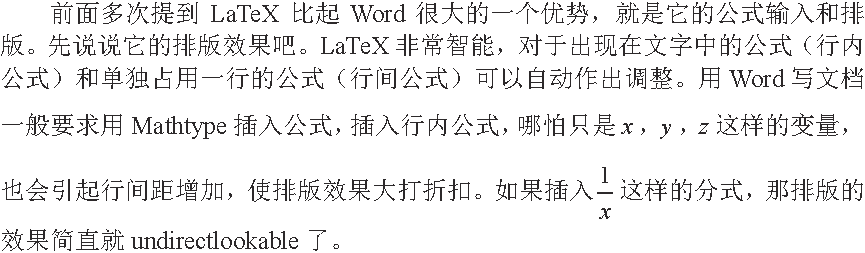
\includegraphics[width=0.9\textwidth]{chapters/wordexample}
\end{center}
\vspace{-1em}
\end{figure}

下面说说在 \LaTeX{} 如何输入公式。
虽然 \LaTeX{} 的公式输入都是靠代码实现,
但 \LaTeX{} 输入公式的语法非常简单,
甚至可以说,以英文为母语的人只要会读,就可以把公式写出来。
先看看下面这个公式
$$  \int_{-1}^{1} \frac{f(x)}{\sqrt{1-x^2}}\,\mathrm{d}x
   =\frac{\pi}{n}\sum_{k=1}^{n}f\left(\cos\frac{2k-1}{2n}\pi\right)
   +\frac{\pi}{2^{2n-1}(2n)!}f^{2n}(\theta) $$
看起来有点小复杂吧。
别急,只要稍加说明,打出比这更复杂的公式都是很简单的事情。

首先,需要学会开始一个公式。
最基础的 \LaTeX{} 中,要输入行内公式,应该这样做 \verb|$行内公式$|。
如果公式比较重要,或者形式比较复杂,
则一般写成行间公式的形式 $$\verb|$$行间公式$$|$$
前面出现的公式就是一个行间公式,我们也可以把它改写成行内公式的形式,效果是这样的
$  \int_{-1}^{1} \frac{f(x)}{\sqrt{1-x^2}}\,\mathrm{d}x
  =\frac{\pi}{n}\sum_{k=1}^{n}f\left(\cos\frac{2k-1}{2n}\pi\right)
  +\frac{\pi}{2^{2n-1}(2n)!}f^{2n}(\theta) $。
与其行间公式形式比较,\LaTeX{} 自动调整了字体大小,
并将求和上下限的位置改写到求和符号的右边以减小竖直方向的空间占用,保持行距。
虽然这样复杂的公式很少有人将它写成行内形式,
但也可以想象一下在 Word 里插入这样复杂的行内公式,
排版效果会变得多么糟糕。

学会了开始公式,我们学习最简单的表达式。
数字和变量直接输入就行,例如 \verb|$2x$| 就可以输出 $2x$ 了。
希腊字母怎么读就怎么输,\verb|$\alpha\beta\gamma$|
就可以输出 $\alpha\beta\gamma$ 了。
大写字母只要开头大写就行,输入 \verb|$\Delta\Phi\Psi$|
就能输出 $\Delta\Phi\Psi$。
等等,还有个小问题,有些字母是有变体的,需要在命令前加 \verb|var|。
如输入 \verb|$\varepsilon\varphi\varPhi\varPsi$|
就得到了 $\varepsilon\varphi\varPhi\varPsi$。

还有各种算符,算符需要用数学正体表示,以区别于变量。
\LaTeX{} 已经定义了很多算符命令,比如 \verb|$\lim,\ln,\sin,\cos$|
得到输出 $\lim,\ln,\sin,\cos$。
还有积分符号 $\int$:\verb|$\int$|,求和符号 $\sum$:\verb|$\sum$| 等,
别忘还有了我们前面自定义的微分算子 $\diff$:\verb|$\diff$|。
现在你应该能理解前面输入的命令 \verb|$\int\sin x\,\diff x$|
是怎样被翻译成公式 $\int\sin x\,\diff x$ 的了吧?
等等 \verb|\,| 是做什么的?
忘了说了,数学模式下空格是被自动忽略的,
输入 \verb|\,| 让 $\sin x$ 和 $\diff x$ 之间隔开一点
(具体说是六分之一空格),会比较好看哦,
如果没有它就变成了 $\int\sin x\diff x$, 是不是有点别扭呢。
另外,加号减号键盘上就有,乘号就是 \verb|\times|, 除号嘛,自己百度吧,反正我从没用过。
还有各种等号不等号,等于,大于小于,键盘上就有。
至于不等号,只要记住,等于是 \verb|eq|, 大于是 \verb|g|,小于是 \verb|l|,
那不等号就是 \verb|\neq|, 大于等于和小于等于分别是 \verb|\geq/\leq|,
远大于远小于就是 \verb|\gg/\ll|,是不是很简单。
当然,\LaTeX{} 还支持更多你见过或者没见过的字符,可以参考 \textit{symbols\/} 文档。

至于上下标,分别用 \verb|^{上标}| 和 \verb|_{下标}| 来输入。
上下标的运用是非常灵活的。
除了各种变量,数字,希腊字母的右侧可以输入上下标,左侧也可以输入,
即使没有字母也可以输入,甚至算符也可以有上下标,积分和求和的上下标分别是他们的上下限。
注意,上下标必须在公式模式下使用。
公式里还可以输入文字 $$\verb|$\text{公式中的文字}$|$$ 就可以插入文字了。
如果你要将一段文字上标,只要 $\scriptsize ^{\verb|$^{\text{上标文字}}$|}$ 就可以了。

还有一些多元运算符。比如分式 \verb|\frac{分子}{分母}| 就可以输入分式。
再比如开 $n$ 次根号的表达式 \verb|\sqrt[n]{数字,变量或表达式}|,
其中 \verb|[n]| 是可选参数,没有时显然就是开平方根啦。


现在,回头看看那个复杂的公式,它的代码是这样的

{\small\vspace{-0.2em}
\begin{verbatim}
 $$ \int_{-1}^{1} \frac{f(x)}{\sqrt{1-x^{2}}}\,\diff x
   =\frac{\pi}{n}\sum_{k=1}^{n}f\left(\cos\frac{2k-1}{2n}\pi\right)
   +\frac{\pi}{2^{2n-1}(2n)!}f^{2n}(\theta) $$
\end{verbatim}}

\vspace{-0.6em}\noindent
应该不难理解吧。


\subsection{带编号的公式}

使用 \verb|$| 和 \verb|$$| 引导公式是 \TeX{} 提供的最基本功能。
\LaTeX{} 提供了更加全面的公式环境,帮助排版各种复杂的公式。
首先是自动编号的公式环境。
利用

{%\small\vspace{-0.2em}
\begin{verbatim}
                   \begin{equation}
                     公式代码
                   \end{equation}
\end{verbatim}}

\vspace{-0.4em}\noindent
即可生成带编号的公式,进而进行交叉引用,这在后面会提到。
如果把 \verb|equation| 替换为 \verb|equation*|,
则排版出不带编号的公式。


\subsection{多行公式}

仅多行公式可以利用 \verb|gather| 环境实现

{
\begin{verbatim}
                   \begin{gather}
                     公式代码1 \\
                     公式代码2
                   \end{gather}
\end{verbatim}}

\vspace{-0.4em}\noindent
同样,如果不需要公式编号,也只需在 \verb|gather| 后加 \verb|*| 即可。
如果仅某行公式不需要编号,
可以在公式代码末尾,换行符号之前利用 \verb|\nonumber| 命令取消编号。

有时候,几行公式需要在等号处对齐,可使用 \verb|align| 环境。
配合对齐符号 \verb|&| 即可实现公式内的对齐。
{
\begin{verbatim}
                   \begin{align}
                     x &= 公式代码1 \\
                       &= 公式代码2
                   \end{align}
\end{verbatim}}

\vspace{-0.4em}\noindent
对公式编号的处理与 \verb|gather| 环境是相同的。

最基本的公式输入就介绍到这里。


\section{插图、表格及其他}

关于插图、表格及其他,说起来甚为繁复,
但掌握 \LaTeX{} 最基本的一些概念后,学起来应该不难。
如有需要,可以参见项目主页上提供的一些教程。


\chapter{模板使用说明}

\section{模板的宗旨}

我们已经知道,\LaTeX{} 通过命令和环境实现各种复杂的排版效果。
在导言区,我们可以通过调入宏包,
利用调入宏包提供的各种设置命令以及自定义各种命令,
来定制文档的排版效果。
如果导言区有很多内容,有时我们把它写在另外一个~.tex 文件中,
利用 \verb|\input{文件}| 的方式调入到导言区中。
这样做的好处是精简文档代码,尽量把内容与自定义设置分开。
在书写某些大型的文档时,
我们也可以使用 \verb|\input{章节文件.tex}| 的方式对文档进行拆分。
编译时只需要调入正在编辑的章节内容,而不必编译整份文档,节约编译的时间。
当然,利用命令 \verb|\input{章节文件.tex}| 来拆分文档有相当的局限性,以后再作说明。

对于比较复杂的模板,更好的方法是将自定义的内容制作成宏包或者文类。
文类可以提供选项,这样一个文类可以根据不同的选项提供不同的排版。
文类中可以方便地重定义某些 \LaTeX{} 的内部命令,来改变排版效果。
更重要的,对于我这样的菜鸟,用文类写模板看起来似乎更加专业一些。
好吧,其实除了看起来更专业我真的没觉得用文类能比 \verb|\input{}| 优越太多。

当然,毕业论文模板另一个相当重要的功能就是提供其他用户一些命令,
以方便地排版出封面、摘要等内容。
用模板排版封面、摘要等内容,无论质量还是方便性,与 Word 相比都有巨大的优势。

\section{开始}

使用本模板,方法十分简单。
我们已经知道怎样开始一个标准的 \LaTeX{} 文档,
使用本模板,只需要把调用的文类替换成 \verb|NJUbachelor| 即可。

{\small\vspace{-0.2em}%
\begin{verbatim}
              \documentclass[参数]{NJUbachelor}
                导言区
              \begin{document}
                正文
              \end{document}
\end{verbatim}}


\section{参数}

你可以直接调用模板而不给出任何参数,缺省选项是为最通用的情况设置。
当然,你也可以根据自己的需求输入参数,来改变缺省设置。
可选的参数有
\begin{description}
  \item[thesis/design] 封面页显示“本科毕业论文”或者“本科毕业设计”。
    其中 \texttt{thesis} 为缺省设置。
  \item[oneside/twoside] 设置单面或者双面打印。
    双面打印会区分单双页,页眉和左右页边距都会根据单双页自动调整。
    双面打印时还会在必要的地方插入空白页。
    其中 \texttt{oneside} 为缺省设置。
  \item[pageheader/nopageheader] 设置是否打印页眉。
    \texttt{nopageheader} 为缺省设置。
  \item[chapter/nochapter] 设置是否支持章 \verb|\chapter{}| 层次。
    不使用章层次更符合学校要求。
    不使用章层次时,最高一级标题是 \verb|\section{节标题}|。
    节标题套用学校章的要求使用四号黑体。
    (简单的说,就是学校要求中的章模板中由 \verb|\section{}| 命令给出)
    毕竟本科学位论文还没有长到要用 \LaTeX{} 中的章层次的地步。
    如果用章层次,则每一章都会另起一页开始。
    使用章层次将无法在正文生成中文标题,
    中文标题的格式三号宋体加粗被套用给章,
    而节的格式仍然是四号黑体。
    其中 \texttt{nochapter} 为缺省设置。
  \item[openright/openany] 如果有章层次,
    设置章层次可在任意页新起一页或者必须在右手(奇数)页新起一页。
    其中 \texttt{openright} 为缺省设置。
  \item[longtitle/shorttitle/manualtitle]
    设置标题页和中文摘要纸的中文标题排版效果。
    长标题可支持自动换行,左对齐显示;
    短标题适合单行标题,可在横线上居中显示;
    手动标题可以利用 \verb|\mtitle| 命令提供手动换行支持,
    每一行标题都可以在横线上居中显示。
    其中 \texttt{longtitle} 为缺省设置。
  \item[shortdepspe/longdepspe]
    你可以根据自己院系和专业名的总长度进行选择。
    选择 shortdepspe 的排版效果和学校给出的中文摘要页是一样的;
    如果院系专业名太长,可以选择 longdepspe 选项。
    其中 \texttt{shortdepspe} 为缺省设置。
  \item[defaultmath/mathptm/mathtxf] 你可以根据自己的喜好选择数学字体。
    其中 \texttt{defaultmath} 为缺省设置。
\end{description}


\section{基本信息输入}

论文基本信息的输入必须在生成标题页和摘要页之前(这似乎很显然)。
建议你在导言区输入论文的基本信息,
以便你的论文信息可以正确写入生成 pdf 的文件属性。
根据学校所给标题页和中英文摘要纸的要求,
本模板定义了以下命令来给出论文的基本信息。
关于基本信息的输入,可以参考 start.tex,这里就不赘述了。

唯一值得注意的,如果需要手动换行,除使用 \textbf{manualtitle} 选项,
另需添加一条命令
$$ \verb|\mtitle{标题1,标题2,标题3}| $$
告诉系统断行方案。
封面页和中文摘要纸将采用相同的断行方案。


\section{正文前内容}

正文前内容包括封面,中英文摘要纸和目录。
首先,封面页由命令 $$ \verb|\makectitlepage| $$ 生成。
它将自动把导言区输入的论文基本信息填写到封面相应的空缺处。
然后分别是中英文标题页,它们分别由中英文摘要环境给出

{\vspace{-0.2em}%
\begin{verbatim}
            \begin{cabstract}      \begin{eabstract}
              中文摘要。              English abstract.
            \end{cabstract}        \end{eabstract}
\end{verbatim}}

\vspace{-0.2em}\noindent
你只需要在环境中写入摘要的内容,
摘要纸的其它空缺同样会依据导言区给出的基本信息自动进行填充。
最后是目录。
学校规定非正文内容要用大写罗马数字作页码。
所以首先利用命令 \verb|\pagenumbering{Roman}| 规定页眉格式。
同时目录页是不需要页眉的,
因此使用 \verb|\thispagestyle{plain}| 规定页面样式为无页眉。
如果使用的是 nochapter 模式,
目录标题作为节层次,摆放的位置会略微偏高,影响美观,
可以试着插入一条 \verb|\vspace*{0em}| 命令。
为了让生成 pdf 的标签带有目录这一条目,
再插入命令 \verb|\pdfbookmark[0]{目录}{contents}|。
最后,是正式的目录生成命令 $$\verb|\tableofcontents|$$
至此,正文前的内容就全部输入完成了。


\section{正文书写}

正文需要另起一页并用阿拉伯数字编号页码,
需要用到命令 \verb|\newpage| 和 \verb|\pagenumbering{arabic}|。
正文第一页一般同样无页眉,因此再跟一条命令 \verb|\thispagestyle{plain}|。
接着,生成正文标题 $$\verb|\makectitle|$$
需要注意的是,chapter 模式下我强行把这一命令设置为空,
即使使用也无法得到输出。
同时,这一模式下我把标题的格式赋给了章标题。
因此 chapter 模式并不很符合学校所给文件的要求。

接着,就可以书写论文正文了。
根据个人的使用经验,为了方便,这里还给出了三个常用的自定义命令。
\begin{description}
  \item[\texttt{\textbackslash{}diff}]
    定义了微分算符,用法前面已经提到。
  \item[\texttt{\textbackslash{}scite\{citekey\}}]
    用以提供参考文献引用的上标效果。
  \item[\texttt{\textbackslash{}unit\{UNIT\}}]
    定义了单位命令,如输入 \verb|5\unit{cm^{2}}|,
    得到 5\unit{cm^{2}},单位自动写成正体,并与数字空开一点距离。
\end{description}

\section{正文后内容}

正文后内容也需要用 \verb|\newpage| 另起一页,
并用 \verb|\pagenumbering{Roman}| 设置页码为大写罗马数字。
正文后内容包括参考文献,致谢和附录。

参考文献的排版方式有两种。
一种是利用 \verb|thebibliography| 环境来实现,
其实现方法如下

{\vspace{-0.2em}%
\begin{verbatim}
            \begin{thebibliography}{n}
              \bibitem{citekey1} bibitem1
              \bibitem{citekey2} bibitem2
                ...  ...  ...  ...  ...
            \end{thebibliography}
\end{verbatim}}

\vspace{-0.2em}\noindent
其中数字 \texttt{n} 的位数应与参考文献条目数的位数相同。
如你有18条参考文献,则 \texttt{n} 可以是任何两位数。
这个参数用于参考文献前数字的对齐。
\texttt{citekey1} 和 \texttt{citekey2} 是参考文献的引用标记,
你可以把 \texttt{bibitem1} 和 \texttt{bibitem2}
按照一定的格式,手动替换成你的参考文献条目。

另一种方法是使用 bibtex 管理参考文献。
模板附带了 bibtex 样式文件 NJUbachelor.bst,
系统可以按照样式文件的定义,自动排版文献数据库并得到参考文献列表。
bibtex 系统的使用在此就不赘述了,感兴趣的同学可以自行百度。

致谢的生成也十分简单,利用命令 $$\verb|\ack|$$
系统就会新起一页,并生成致谢标题。
在 chapter 模式下,致谢标题的等级为章,nochapter 模式下则为节,
并自动套用章或节的标题格式。
你只需在该命令后直接书写致谢的内容即可。

书写附录,需要另起一页,
在 nochapter 模式下需要额外的 \verb|\newpage| 命令。
在 chapter 模式下,因为章节标题自动新起一页,所以就无需手动分页了。
在命令 $$\verb|\appendix|$$ 后开始附录。
附录的章节标题及内容的书写与正文并无差别,只是编号的形式会作调整。

至此,怎样使用该模板书写毕业论文,也基本讲解完了。

%\chapter{}

“太湖美,美就美在太湖水……”昔日描绘美丽江南水乡母亲湖的优美歌谣只能留在人们的记忆中了,如今,当太湖流域的人们再唱起这首歌的时候,却是另一番滋味。党的十七大的召开,为寻求解决太湖蓝藻污染提供了契机。继物质文明、精神文明、政治文明之后,党的十七大报告中首次提出“建设生态文明”,把我国的社会主义文明建设提高到了一个全新高度。“建设生态文明,基本形成节约能源资源和保护生态环境的产业结构、增长方式、消费模式”。显然生态环境已成为十七大报告所描绘的中国小康社会图景的重要组成部分,特别是将人与自然和谐相处的关系纳入到社会发展目标中统筹考虑。毋容置疑,将人与自然的关系纳入到社会发展目标中统筹考虑,建设生态文明,不仅是中国共产党对子孙后代和世界负责的庄重承诺,也为人们治理太湖蓝藻树立了信心和提供了新的思路。治理太湖污染的工作已经开展多年,为何这个“固疾”却久治不愈?显然与人们传统思想道德观念中的人类中心主义思想是分不开的。太湖水污染的现状要想真正得到改善,人们也应该转变原有的环境伦理观念了,实现由人类中心主义向生态中心主义的转变。

\section{中文节 English Section}

\newpage

{\heiti 中文 English}

\chapter{第一章}

\section{这是第一节}

%\makectitle

 “太湖美,美就美在太湖水……”昔日描绘美丽江南水乡母亲湖的优美歌谣只能留在人们的记忆中了,如今,当太湖流域的人们再唱起这首歌的时候,却是另一番滋味。党的十七大的召开,为寻求解决太湖蓝藻污染提供了契机。继物质文明、精神文明、政治文明之后,党的十七大报告中首次提出“建设生态文明”,把我国的社会主义文明建设提高到了一个全新高度。“建设生态文明,基本形成节约能源资源和保护生态环境的产业结构、增长方式、消费模式”。显然生态环境已成为十七大报告所描绘的中国小康社会图景的重要组成部分,特别是将人与自然和谐相处的关系纳入到社会发展目标中统筹考虑。毋容置疑,将人与自然的关系纳入到社会发展目标中统筹考虑,建设生态文明,不仅是中国共产党对子孙后代和世界负责的庄重承诺,也为人们治理太湖蓝藻树立了信心和提供了新的思路。治理太湖污染的工作已经开展多年,为何这个“固疾”却久治不愈?显然与人们传统思想道德观念中的人类中心主义思想是分不开的。太湖水污染的现状要想真正得到改善,人们也应该转变原有的环境伦理观念了,实现由人类中心主义向生态中心主义的转变。

\section{太湖蓝藻事件及蓝藻带来的危害}

\subsection{太湖蓝藻事件及蓝藻带来的危害}

\subsubsection{太湖蓝藻事件及蓝藻带来的危害}

太湖作为本流域的开放型水体,接纳一些大河携带了苏、锡、常、湖四个市大量的工农业废水和生活污水入湖,随着太湖地区人口的增加和经济的发展,太湖受到了越来越严重的污染。水中溶解氧在减少,化学耗氧量和氨氮在增加,富营养化急速发展。近年来的研究表明,太湖是有机物和营养物污染型湖泊,由各种途径进入湖体的污染物有26种,影响太湖水质的主要污染物为氮(凯氏氮)、磷和高锰酸钾指数(CODMn)[1] 。这些主要的污染物为藻类生长提供了充足的养分。近年来蓝藻已成为太湖的常客,每到夏天蓝藻都有不同程度的暴发。从2007年4月开始,太湖流域高温少雨,太湖水位正常偏低,梅梁湖等湖湾出现大规模蓝藻现象,无锡市太湖饮用水水源地受到严重威胁。从2007年5月29日晚开始,江苏省无锡市的自来水开始出现变味发臭等现象,市民生活用水受到影响。无锡市民开始抢购纯净水,人们开始变得不安和恐慌起来。

\newpage

“太湖美, 美就美在太湖水……”昔日描绘美丽江南水乡母亲湖的优美歌谣只能留在人们的记忆中了, 如今, 当太湖流域的人们再唱起这首歌的时候, 却是另一番滋味。党的十七大的召开, 为寻求解决太湖蓝藻污染提供了契机。继物质文明、精神文明、政治文明之后, 党的十七大报告中首次提出“建设生态文明”, 把我国的社会主义文明建设提高到了一个全新高度。“建设生态文明, 基本形成节约能源资源和保护生态环境的产业结构、增长方式、消费模式”。显然生态环境已成为十七大报告所描绘的中国小康社会图景的重要组成部分, 特别是将人与自然和谐相处的关系纳入到社会发展目标中统筹考虑。毋容置疑, 将人与自然的关系纳入到社会发展目标中统筹考虑, 建设生态文明, 不仅是中国共产党对子孙后代和世界负责的庄重承诺, 也为人们治理太湖蓝藻树立了信心和提供了新的思路。治理太湖污染的工作已经开展多年, 为何这个“固疾”却久治不愈?显然与人们传统思想道德观念中的人类中心主义思想是分不开的。太湖水污染的现状要想真正得到改善, 人们也应该转变原有的环境伦理观念了, 实现由人类中心主义向生态中心主义的转变。

“太湖美, 美就美在太湖水……”昔日描绘美丽江南水乡母亲湖的优美歌谣只能留在人们的记忆中了, 如今, 当太湖流域的人们再唱起这首歌的时候, 却是另一番滋味。党的十七大的召开, 为寻求解决太湖蓝藻污染提供了契机。继物质文明、精神文明、政治文明之后, 党的十七大报告中首次提出“建设生态文明”, 把我国的社会主义文明建设提高到了一个全新高度。“建设生态文明, 基本形成节约能源资源和保护生态环境的产业结构、增长方式、消费模式”。显然生态环境已成为十七大报告所描绘的中国小康社会图景的重要组成部分, 特别是将人与自然和谐相处的关系纳入到社会发展目标中统筹考虑。毋容置疑, 将人与自然的关系纳入到社会发展目标中统筹考虑, 建设生态文明, 不仅是中国共产党对子孙后代和世界负责的庄重承诺, 也为人们治理太湖蓝藻树立了信心和提供了新的思路。治理太湖污染的工作已经开展多年, 为何这个“固疾”却久治不愈?显然与人们传统思想道德观念中的人类中心主义思想是分不开的。太湖水污染的现状要想真正得到改善, 人们也应该转变原有的环境伦理观念了, 实现由人类中心主义向生态中心主义的转变。

“太湖美, 美就美在太湖水……”昔日描绘美丽江南水乡母亲湖的优美歌谣只能留在人们的记忆中了, 如今, 当太湖流域的人们再唱起这首歌的时候, 却是另一番滋味。党的十七大的召开, 为寻求解决太湖蓝藻污染提供了契机。继物质文明、精神文明、政治文明之后, 党的十七大报告中首次提出“建设生态文明”, 把我国的社会主义文明建设提高到了一个全新高度。“建设生态文明, 基本形成节约能源资源和保护生态环境的产业结构、增长方式、消费模式”。显然生态环境已成为十七大报告所描绘的中国小康社会图景的重要组成部分, 特别是将人与自然和谐相处的关系纳入到社会发展目标中统筹考虑。毋容置疑, 将人与自然的关系纳入到社会发展目标中统筹考虑, 建设生态文明, 不仅是中国共产党对子孙后代和世界负责的庄重承诺, 也为人们治理太湖蓝藻树立了信心和提供了新的思路。治理太湖污染的工作已经开展多年, 为何这个“固疾”却久治不愈?显然与人们传统思想道德观念中的人类中心主义思想是分不开的。太湖水污染的现状要想真正得到改善, 人们也应该转变原有的环境伦理观念了, 实现由人类中心主义向生态中心主义的转变。

\noindent
This is English test:

When baking in a rectangular pan heat is concentrated in the 4 corners and the product gets overcooked at the corners (and to a lesser extent at the edges). In a round pan the heat is distributed evenly over the entire outer edge and the product is not overcooked at the edges. However, since most ovens are rectangular in shape using round pans is not efficient with respect to using the space in an oven.

\sf
When baking in a rectangular pan heat is concentrated in the 4 corners and the product gets overcooked at the corners (and to a lesser extent at the edges). In a round pan the heat is distributed evenly over the entire outer edge and the product is not overcooked at the edges. However, since most ovens are rectangular in shape using round pans is not efficient with respect to using the space in an oven.

\bf
When baking in a rectangular pan heat is concentrated in the 4 corners and the product gets overcooked at the corners (and to a lesser extent at the edges). In a round pan the heat is distributed evenly over the entire outer edge and the product is not overcooked at the edges. However, since most ovens are rectangular in shape using round pans is not efficient with respect to using the space in an oven.

\it
When baking in a rectangular pan heat is concentrated in the 4 corners and the product gets overcooked at the corners (and to a lesser extent at the edges). In a round pan the heat is distributed evenly over the entire outer edge and the product is not overcooked at the edges. However, since most ovens are rectangular in shape using round pans is not efficient with respect to using the space in an oven.

\sl
When baking in a rectangular pan heat is concentrated in the 4 corners and the product gets overcooked at the corners (and to a lesser extent at the edges). In a round pan the heat is distributed evenly over the entire outer edge and the product is not overcooked at the edges. However, since most ovens are rectangular in shape using round pans is not efficient with respect to using the space in an oven.

\rm
ABCDEFGHIJKLMNOPQRSTUVWXYZabcdefghijklmnopqrstuvwxyz

\sf
ABCDEFGHIJKLMNOPQRSTUVWXYZabcdefghijklmnopqrstuvwxyz

\it
ABCDEFGHIJKLMNOPQRSTUVWXYZabcdefghijklmnopqrstuvwxyz

\sl
ABCDEFGHIJKLMNOPQRSTUVWXYZabcdefghijklmnopqrstuvwxyz

\bf
ABCDEFGHIJKLMNOPQRSTUVWXYZabcdefghijklmnopqrstuvwxyz

\rm

\begin{figure}[htb]
\caption{Hello}
\label{fig}
\end{figure}

\autoref{fig}

\begin{equation}
\int\sin x \,\diff xk \label{eq}
\end{equation}

\autoref{eq}

$$  \int_{-1}^{1} \frac{f(x)}{\sqrt{1-x^2}}\,\mathrm{d}x
   =\frac{\pi}{n}\sum_{k=1}^{n}f\left(\cos\frac{2k-1}{2n}\pi\right)
   +\frac{\pi}{2^{2n-1}(2n)!}f^{2n}(\theta) $$


\backmatter

\newpage
\pagenumbering{Roman}

\nocite{*}
\bibliographystyle{njubachelor}
%\bibliography{refs/articles,refs/books}
\bibliography{refs/jabrefbib}

\ack

感谢物理学院的基友们在模板制作期间给予的鼓励。
特别感谢化学化工学院杨晨同学帮助我完成了 Mac 平台的测试工作,
并及时地发现了一些 bug 并提出了解决方案,
以及对模板排版效果提出了一些建议。

感谢百度百科,感谢 \CTeX{} 论坛。


\appendix

\chapter{正文拷贝测试}

\songti

感谢物理学院的基友们在模板制作期间给予的鼓励。
特别感谢化学化工学院杨晨同学帮助我完成了 Mac 平台的测试工作,
并及时地发现了一些 bug 并提出了解决方案,
以及对模板排版效果提出了一些建议。

\heiti
感谢物理学院的基友们在模板制作期间给予的鼓励。
特别感谢化学化工学院杨晨同学帮助我完成了 Mac 平台的测试工作,
并及时地发现了一些 bug 并提出了解决方案,
以及对模板排版效果提出了一些建议。

\kaishu
感谢物理学院的基友们在模板制作期间给予的鼓励。
特别感谢化学化工学院杨晨同学帮助我完成了 Mac 平台的测试工作,
并及时地发现了一些 bug 并提出了解决方案,
以及对模板排版效果提出了一些建议。

\fangsong
感谢物理学院的基友们在模板制作期间给予的鼓励。
特别感谢化学化工学院杨晨同学帮助我完成了 Mac 平台的测试工作,
并及时地发现了一些 bug 并提出了解决方案,
以及对模板排版效果提出了一些建议。


\end{document}
